\documentclass[11.5pt, aspectratio=169]{beamer}
\usepackage{amsmath, amssymb, stmaryrd, mathpartir, commath, url, longtable,hyperref,tabularx}

\usepackage{forloop, microtype}
\usepackage{wasysym}
%\usepackage[dvipsnames]{xcolor}
\usepackage{csquotes}
%\usepackage{mathptmx}
\usepackage{listings}
\hypersetup{colorlinks=true,citecolor=blue}
\RequirePackage{subcaption}
\captionsetup{compatibility=false}
\usepackage{graphicx}
\usepackage{xspace}
\usepackage{dirtytalk}
\usepackage{xparse}% http://ctan.org/pkg/xparse
\usepackage{etoolbox}% http://ctan.org/pkg/etoolbox
\newcommand{\lambdacalc}{\ensuremath{\lambda}-calculus\xspace}
\newenvironment{fake}[1]{\par\vspace{3pt}\noindent\textbf{#1}\itshape}{\normalfont\ignorespacesafterend\vspace{3pt}\par}

\usepackage{float}
\floatstyle{boxed}
\restylefloat{figure}
\usepackage{verbatim}

\newcommand{\backupbegin}{
   \newcounter{finalframe}
   \setcounter{finalframe}{\value{framenumber}}
}
\newcommand{\backupend}{
   \setcounter{framenumber}{\value{finalframe}}
}

\setbeamercovered{%
  again covered={\opaqueness<1->{15}}}



% TIKZ STUFF


\usepackage{amsmath,verbatim}

\lstdefinelanguage{Links}{%
  morekeywords={typename, fun, linfun, op, var, if, this, true, false, else, case, switch, handle,
    handler, shallowhandler, open, do, sig, new, send, receive, spawnAt, spawn,
module, request, accept, try, as, in, otherwise, catch, offer, select, raise,
fork, spawnClient, cancel, catch},%
  sensitive=t, %
  comment=[l]{\#\ },%
  escapeinside={(*}{*)},%
  morestring=[d]{"},%
  keywordstyle=\color{blue},
  showstringspaces=false
  %frame = single
 }

% Links style
\lstset{
  basicstyle=\linespread{1.3}\ttfamily\large,
  keywordstyle=\bfseries,
  language=Links,
  backgroundcolor=\color{white}
}


\usepackage{expl3,xparse}
\makeatletter
\let\old@lstKV@SwitchCases\lstKV@SwitchCases
\def\lstKV@SwitchCases#1#2#3{}
\makeatother
\usepackage{lstlinebgrd}
\makeatletter
\let\lstKV@SwitchCases\old@lstKV@SwitchCases

\lst@Key{numbers}{none}{%
    \def\lst@PlaceNumber{\lst@linebgrd}%
    \lstKV@SwitchCases{#1}%
    {none:\\%
     left:\def\lst@PlaceNumber{\llap{\normalfont
                \lst@numberstyle{\thelstnumber}\kern\lst@numbersep}\lst@linebgrd}\\%
     right:\def\lst@PlaceNumber{\rlap{\normalfont
                \kern\linewidth \kern\lst@numbersep
                \lst@numberstyle{\thelstnumber}}\lst@linebgrd}%
    }{\PackageError{Listings}{Numbers #1 unknown}\@ehc}}
\makeatother

\ExplSyntaxOn
\NewDocumentCommand \lstcolorlines { O{green} m }
{
  \clist_if_in:nVTF { #2 } { \the\value{lstnumber} }{ \color{#1} }{\color{white}}
}
\ExplSyntaxOff
\newcommand{\textl}{\text{\lightning}}


\newcommand{\calcwd}[1]{\mathbf{\mathbf{#1}}}
\newcommand{\one}{\mathbf{1}}
\newcommand{\lightningnu}[1]{\nu #1\lightning}
\newcommand{\gvqueue}[4]{#1(#2){\leftrightsquigarrow} #3(#4)}
\newcommand{\mkwd}[1]{\ensuremath{\mathsf{#1}}}
\newcommand{\gvsend}[2]{\calcwd{send} \: #1 \: #2}
\newcommand{\gvrecv}[1]{\calcwd{receive} \: #1}
\newcommand{\gvcancel}[1]{\calcwd{cancel} \app #1}
\newcommand{\gvclose}[1]{\calcwd{close} \app #1}
\newcommand{\gvcancelup}[1]{\calcwd{cancel} \app #1}
\newcommand{\gvout}[2]{!{#1}.{#2}}
\newcommand{\gvin}[2]{?{#1}.{#2}}
\newcommand{\gvend}{\mathsf{End}\xspace}
\newcommand{\gvfork}[1]{\calcwd{fork} \, #1}
\newcommand{\app}{\:}
\newcommand{\inl}[1]{\calcwd{inl} \app #1}
\newcommand{\inr}[1]{\calcwd{inr} \app #1}
\newcommand{\gvcase}[2]{\calcwd{case} \: #1 \: \calcwd{of} \: \{ #2 \}  }
\newcommand{\gvlet}[3]{\calcwd{let} \: #1 = #2 \: \calcwd{in} \: #3}
\newcommand{\tryasinotherwise}[4]{\calcwd{try} \: #1 \: \calcwd{as} \: #2 \: \calcwd{in} \: #3 \: \calcwd{otherwise} \: #4}
\newcommand{\raiseexn}{\calcwd{raise}\xspace}
\newcommand{\un}[1]{\mkwd{un}(#1)}
\newcommand{\gvdual}[1]{\overline{#1}}
%\newcommand{\compat}{\asymp}
\newcommand{\evalperhaps}{\eval^?}
\newcommand{\evalstar}{\eval^*}
\newcommand{\scancel}[1]{\text{\lightning} #1}
\newcommand{\scancelmv}[1]{#1 \lightning}
\newcommand{\config}[1]{\mathcal{#1}}
\newcommand{\seq}[1]{\overrightarrow{#1}}
\newcommand{\fv}[1]{\mathsf{fv}(#1)}
%\newcommand{\fcv}[1]{\mathsf{fcv}(#1)}
\newcommand{\fvs}[1]{\mathsf{fvs}(#1)}
\newcommand{\fn}[1]{\mathsf{fn}(#1)}
\newcommand{\fcvs}[1]{\fn{#1}}
\newcommand{\chansharp}[1]{#1^{\sharp}}
\newcommand{\chanflat}[1]{#1^{\flat}}
\newcommand{\without}{/}
\newcommand{\equivceval}{\equiv \longrightarrow_{\textsf{C}} \equiv}
\newcommand{\cevalthick}{\Longrightarrow_{\textsf{C}}}
\newcommand{\ceval}{\quad \longrightarrow \quad}
\newcommand{\teval}{\longrightarrow_{\textsf{M}}}
\newcommand{\eps}[1]{\mkwd{eps}(#1)}
\newcommand{\affected}[1]{\mkwd{affected}(#1)}
\newcommand{\halt}{\calcwd{halt}\xspace}
\newcommand{\bcirc}{\bullet}
\newcommand{\wcirc}{\circ}
\newcommand{\disable}[1]{\mkwd{disable}(#1)}

\newcommand{\blocked}[2]{\mkwd{blocked}(#1, #2)}
\newcommand{\depends}[3]{\mkwd{depends}(#1, #2, #3)}
\newcommand{\deadlocked}[1]{\mkwd{deadlocked}(#1)}

\newcommand{\Ceval}{\Longrightarrow_{\textsf{C}}}

\newcommand{\dom}[1]{\mkwd{dom}(#1)}

\newenvironment{remark}{\paragraph{Remark.}}{\hfill \tiny{$\square$}}
%\newtheorem{remark}{Remark}
%\newtheorem{lemma}{Lemma}
%\newtheorem{proposition}{Proposition}
%\newtheorem{corollary}{Corollary}
%\newtheorem{definition}{Definition}


\newcommand{\defeq}{\triangleq}

\newcommand{\todo}[1]{{\noindent\small\color{red} \framebox{\parbox{\dimexpr\linewidth-2\fboxsep-2\fboxrule}{\textbf{TODO:} #1}}}}
\newenvironment{subcase}[1]
  {\textbf{Subcase #1} \hfill \\
  \begin{adjustwidth}{0.25cm}{}}
  {\end{adjustwidth}}

\newenvironment{proofcase}[1]
  {\totheleft{\textbf{Case \textsc{#1}}}}
  {}
\newcommand{\lto}{\multimap}
\newcommand{\proofstep}[1]{
  \begin{compactitem}
  \item #1
  \end{compactitem}
}

\newcommand{\names}[1]{\mkwd{names}(#1)}

\arraycolsep=1pt%\def\arraystretch{2.2}

\newcommand{\transl}[1]{\llbracket #1 \rrbracket}
\newcommand{\stranslateb}[1]{\mathcal{S}\llparenthesis #1 \rrparenthesis}
\newcommand{\ttranslateb}[1]{\mathcal{T}\llparenthesis #1 \rrparenthesis}
\newcommand{\etranslateb}[1]{\mathcal{E}\llparenthesis #1 \rrparenthesis}
\newcommand{\ptranslateb}[1]{\mathcal{P}\llparenthesis #1 \rrparenthesis}

\newcommand{\gvoutone}[1]{{!}#1}
\newcommand{\gvinone}[1]{{?}#1}
\newcommand{\letintwo}[2]{\calcwd{let} \: #1 = #2 \: \calcwd{in}}
\newcommand{\totheleft}[1]{\begin{flushleft}#1\end{flushleft}}
\usepackage[T1]{fontenc}
\usepackage[scaled=0.85]{beramono}
\newcommand\doubleplus{+\kern-1.3ex+\kern0.8ex}
\newcommand{\metadef}[1]{\calcwd{#1}}


\newcommand{\runtimechan}[2]{\mkwd{Channel}(#1, #2)}
\newcommand{\closure}[2]{\langle #1, #2 \rangle}
%\newcommand{\boldleft}{\textbf{\{ }}
%\newcommand{\boldright}{\textbf{ \}}}
\newcommand{\contained}[1]{\metadef{Channels}(#1)}

\newcommand{\ba}{\begin{array}}
\newcommand{\ea}{\end{array}}

\newcommand{\bl}{\ba[t]{@{}l@{}}}
\newcommand{\el}{\ea}


\newcommand{\triestosend}[4]{{#1} \xRightarrow[#4]{#2} {#3}}

\newcommand{\notsmall}{}

\newcommand{\oftype}{\,{:}\,}

\newcommand{\sendpair}[2]{\calcwd{send} \: (#1, #2)}

%\renewcommand{\paragraph}[1]{\textbf{\textit{#1}}}
\usepackage{tikz-cd}

\newcommand{\exnty}{\mkwd{Exn}\xspace}
\newcommand{\raiseexnP}[1]{\calcwd{raise} \: #1}
\newcommand{\tryinunless}[4]{\calcwd{try} \: #1 \: \calcwd{as} \: #2 \:
    \calcwd{in} \: #3 \: \calcwd{unless} \: #4}

\newcommand{\handled}[1]{\mkwd{Handled}(#1)}

\newcommand{\highlight}[1]{{\color{colorredorange} #1} }
\newcommand{\highlightpink}[1]{{\color{colorpink} #1} }
\newcommand{\highlightwarning}[1]{{\color{colorlightpink} #1} }
\newcommand{\midspace}{\; \mid{} \; }
\setlength\tabcolsep{1.5em}

\newcommand{\lact}{\lambda_{\text{act}}\xspace}
\newcommand{\lch}{\lambda_{\text{ch}}\xspace}

\usepackage{config/presento}
\usepackage{framed}
\usepackage{stmaryrd}
\usepackage{amsmath}
\usepackage{wasysym}
% Presento style file
\usepackage{float,lipsum}
\floatstyle{boxed}
\usepackage{mathpartir}
% custom command and packages
% custom packages
\usepackage{textpos}
\setlength{\TPHorizModule}{1cm}
\setlength{\TPVertModule}{1cm}

\newcommand\crule[1][black]{\textcolor{#1}{\rule{2cm}{2cm}}}


\usepackage{verbatim}
% Information
\title{FORCE2019 Conference}
\author{Simon Fowler}
\institute{University of Edinburgh}
\date{14th November 2019}

\begin{document}

% Title page
\begin{frame}[plain]
\titlepage


\hfill
\vspace{-1em}
$
\renewcommand*{\arraystretch}{1.8}
\begin{array}{r}
   
\includegraphics[height=0.7cm, keepaspectratio]{images/logos/inf_uoe.png} \\
\end{array}
$
\end{frame}


\begin{frame}{Force11}
  \begin{center}
    
\includegraphics[width=0.6\textwidth]{images/force11.png}
  \end{center}
  \only<1>{
    \begin{center}
    ``FORCE11 is a community of scholars, librarians, archivists, publishers and research funders that has arisen organically to help facilitate the change toward improved knowledge creation and sharing.
    Individually and collectively, we \emph{aim to bring about a change in modern scholarly communications through the effective use of information technology}.''
    \end{center}
    }
    \only<2>{
  \begin{fullpageitemize}
    \item Scholarly research outputs? Traditionally publications.
    \item But there's much more to it:
      \begin{itemize}
        \itemR Software, metadata, semantic linking\ldots
      \end{itemize}
    \item People don't read / order print journals anymore; why are online publications the same as print journals?
  \end{fullpageitemize}
  }
\end{frame}

\begin{frame}{FORCE2019}
  \begin{center}
    
\includegraphics[width=0.8\textwidth]{images/force2019.png}
  \end{center}

  \begin{fullpageitemize}
  \item My take on FORCE conferences: ``The ICFP of the scholarly communications community''
  \item This one was in Edinburgh! So I went. \textasciitilde 200-300 attendees, held at Murrayfield conference centre
    \begin{itemize}
      \itemR (aside: it was \emph{cold})
    \end{itemize}
  \item Remainder of this talk: some interesting talks, and my takeaways
  \end{fullpageitemize}
\end{frame}

\framecard{{\color{white}\bigtext{3 Interesting Talks}}}

\begin{frame}{Perpetual access machines: archiving web-published scholarship at scale \\ {\small Jefferson Bailey and Bryan Newbold}}
  \begin{center}
    
\includegraphics[width=0.2\textwidth]{images/internet-archive.png}
  \end{center}

  \begin{fullpageitemize}
    \item Internet Archive (\url{http://www.archive.org}): Keeps snapshots of web content
    \item \textbf{Idea:} Use this for scholarly output, too
      \begin{itemize}
        \itemR ``At risk'' scholarship, especially non-English-language
        \itemR Crawls, gathers metadata, checks whether PDFs are scholarly outputs
        \itemR Prioritises informally published works (we hope DL will be around for a while!)
      \end{itemize}
  \end{fullpageitemize}
\end{frame}

\begin{frame}{Transparent peer review: a collaborative approach to opening and building the scholarly record \\ {\small Laura Simonite}}
  \begin{center}
    
\includegraphics[width=0.35\textwidth]{images/Publons_logo.png}
  \end{center}

  \begin{fullpageitemize}
    \item Peer review works out in the end, but often problematic
      \begin{itemize}
        \itemR Reviewer 2
        \itemR ``This will be a short and superficial review because my intended subreferee dropped out\ldots''
      \end{itemize}
    \item Authors opt-in to transparent peer review; reviews shown along with paper, assigned DOIs
    \item I'm conflicted. Good idea, but I'm not sure about having my reviews available to all\ldots
  \end{fullpageitemize}
\end{frame}

\begin{frame}[fragile]{The Journal of Open Source Software: when collaborative open source meets peer review\\ {\small Arfon Smith}}
  \begin{center}
    
\includegraphics[width=0.4\textwidth]{images/joss.jpg}
  \end{center}

  \begin{fullpageitemize}
    \item Open access journal about open-source software
      \begin{itemize}
        \itemR Short, citable papers
        \itemR Quality control on both software \emph{and} paper
      \end{itemize}

    \item Review process open, on GitHub
      \begin{itemize}
        \itemR Facilitated by a bot called \verb+@whedon+ :)
      \end{itemize}

    \item In my opinion, the best talk of the conference
  \end{fullpageitemize}

\end{frame}

\framecard{{\color{white}\bigtext{Takeaways}}}

\begin{frame}{Takeaways}

  \begin{fullpageitemize}
\item {\large {\textbf{Takeaway 1: } Embrace persistent IDs}}
      \begin{itemize}
        \itemR ORCID: Unique researcher identifier. Associates your work with you, even through name changes, etc.
         % (Rendering is awful in LNCS, but no other negatives.)
        \itemR DOIs: Not just for papers, but for \emph{any} sort of digital object
      \end{itemize}
      \vspace{0.5em}
      \pause

    \item { \large {\textbf{Takeaway 2: }} Follow correct software citation practices }
      \begin{itemize}
        \itemR Cite and give credit for essential software. Checklists available
        %\itemR If authoring software, provide a way for people to cite your software
        %\itemR Various checklists out there already
      \end{itemize}
      \vspace{0.5em}
      \pause

    \item { \large {\textbf{Takeaway 3: }} arXiv for preprints, not transient website links}
      \begin{itemize}
        \itemR People should be able to cite a specific \emph{version} of your paper
      \end{itemize}
      \vspace{0.5em}
      \pause

    \item {\large {\textbf{Takeaway 4: }} Archive and DOI your supplementary material!}
      \begin{itemize}
        \itemR Data / software artifacts are \emph{important parts of your output}
        \itemR Archive them and get DOIs: use figshare / Zenodo for example
      \end{itemize}
      \vspace{0.5em}
      \pause

    \item { \large {\textbf{Takeaway 5: }} Open access is the future!}
      \begin{itemize}
        \itemR Closed access papers are not REF-able. It's on its way out.
        \itemR Still some confusion as to sustainability.
      \end{itemize}
  \end{fullpageitemize}
\end{frame}

\begin{frame}{Practicing, preaching, and all that\ldots}
  \begin{center}
  \only<1>{
    
\includegraphics[width=0.65\textwidth]{images/arxiv.png}
  }
  \only<2>{
    
\includegraphics[width=0.5\textwidth]{images/orcid.png}
  }
  \only<3>{
    
\includegraphics[width=0.5\textwidth]{images/figshare-citation.png}
    \vspace{2em}

    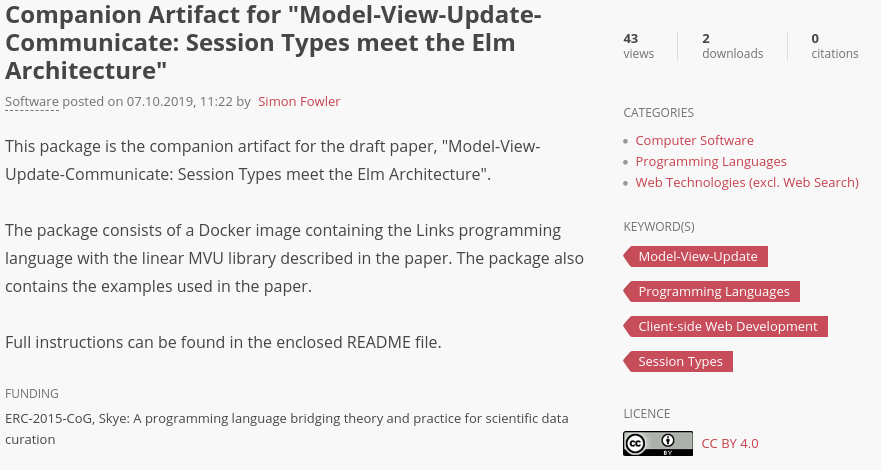
\includegraphics[width=0.65\textwidth]{images/figshare.png}
  }
\end{center}
\end{frame}

\begin{frame}{Fin}
  \begin{fullpageitemize}
    \item FORCE conferences: Discussion of future of scholarly communication
    \item Murrayfield conference centre is freezing, but conference was interesting
    \item {\large \textbf{Takeaways:}}
      \begin{itemize}
        \item 1. Embrace persistent IDs
        \item 2. Follow correct software citation practices
        \item 3. ArXiv your preprints
        \item 4. Archive your supplementary material
        \item 5. Open access is the future!
      \end{itemize}
  \end{fullpageitemize}

  \begin{center}
    Thanks! Questions?
  \end{center}
\end{frame}

\end{document}
